\documentclass[twoside,10pt]{article}
\usepackage{shlists}
\usepackage[spanish]{babel}
\usepackage[applemac]{inputenc}
\usepackage[T1]{fontenc}

\usepackage{multicol}
\usepackage{picinpar}

\usepackage{url}
\newcounter{vol}
\newcounter{num}
\newcounter{anyo}
\setcounter{vol}{8}
\setcounter{num}{1}
\setcounter{anyo}{2015}
\newcommand{\mes}{Enero}
\usepackage{revisionNLcol}


\title{Docencia 2.0\\ \large Juan Juli\'an Merelo, Fernando 
Tricas}
\author{\LARGE La ciencia, la ingenier\'{\i}a y la cultura}


\date{}

\AutTit{Docencia 2.0}

\begin{document}
\addtocounter{page}{2}

\maketitle
\vspace*{-8ex}

\begin{multicols}{2}
En general, en cualquier carrera se ense\~na la teor\'{\i}a y la pr\'actica
relacionada con la misma, obviando aspectos humanos, emocionales o
culturales. Si se ense\~na un lenguaje de programaci\'on o las estructuras de
datos que se usan en \'el o los algoritmos o, para el caso, cualquier otra
cosa, no se hace \'enfasis en aspectos humanos, ni culturales, ni laborales.
En realidad, pr\'acticamente nada de esas habilidades horizontales con
las que tanto nos tuvimos que pelear cuando elaboramos los planes de
estudios de Bolonia.
El problema es que, cada vez m\'as, esos aspectos culturales son m\'as
dif\'{\i}ciles de desligar de los puramente t\'ecnicos. Metodolog\'{\i}as de desarrollo
como SCRUM son m\'as culturales que t\'ecnicas: se trata de una forma de
organizar los equipos de trabajo e interactuar con los compa\~neros, m\'as
que una serie de
herramientas o de t\'ecnicas. DevOps, el arte de colocar conjuntamente a los
encargados de sistemas, de calidad y de desarrollo trabajando conjuntamente
sobre un mismo repositorio de c\'odigo es m\'as un cambio cultural,
organizativo, que t\'ecnico: pasar de tres departamentos separados a un s\'olo
equipo de trabajo que incluye los tres aspectos. 
En parte, estos cambios han surgido por la adopci\'on de sistemas basados en
la nube. Sistemas no instala ya un ordenador y un servidor para los
desarrolladores, provisiona instancias para diferentes tareas y tiene que
hacerlo de forma continua. La adopci\'on de m\'etodos de integraci\'on y
lanzamiento continuo (CI/CD) tambi\'en hace que los ciclos de prueba del
software sean r\'apidos y, de hecho, se hagan tambi\'en en la nube en
servidores de CI que ejecutan Jenkins o alg\'un software similar. El
despliegue, que podr\'{\i}a ser antes la parcela de una parte especializada del
equipo de sistemas o de desarrollo, se hace ahora usando herramientas tales
como Fabric o Foreman, programadas por el mismo equipo integrado.
Es complicado reflejar esto en la ense\~nanza universitaria, que es lo que
nos ocupa, porque generalmente refleja esa compartimentalizaci\'on que
aparece en la empresa. Las asignaturas de ``sistemas'' no hablan con las de
``desarrollo'' y estas no hablan con las de ``Ingenier\'{\i}a del
Software''. El
resultado es un choque cultural de los graduados cuando se incorporan a
alguna compa\~n\'{\i}a moderna, una \textsl{startup} que tenga un equipo de desarrollo
\'agil, y se encuentre que ni se usa UML ni siempre el mismo lenguaje ni su
labor es desarrollar, sino testear o escribir los \textsl{hooks} que se tienen que
ejecutar cada vez que se env\'{\i}e c\'odigo al repo.
Afortunadamente, los tiempos est\'an cambiando. Muchos grados adoptan
proyectos integrados que permiten a los alumnos desarrollar pr\'acticas y
trabajos fin de grado en un entorno m\'as real; las asignaturas se ponen de
acuerdo en integrar sus pr\'acticas para echar abajo los cub\'{\i}culos en las que
pueden haberse convertido. Y, finalmente, los alumnos tambi\'en aprenden a
ser m\'as flexibles y a adoptar buenas pr\'acticas desde la escritura de la
primera l\'{\i}nea de c\'odigo.
En resumen, los profesores estamos aprendiendo a incorporar esa cultura y a
que los alumnos aprendan de ella. Poco a poco.
Cuando se dan este tipo de integraciones no s\'olo se pueden mejorar la
relaci\'on de los conocimientos que proporcionan las
 diferentes materias, sino que se pueden a\~nadir las habilidades
 relacionadas con la organizaci\'on y gesti\'on de proyectos y
 tambi\'en las relacionadas con la comunicaci\'on, negociaci\'on, e
 interacci\'on con el ``mundo exterior''.  No se trata s\'olo de las
 tareas relacionadas con la superaci\'on de la asignatura ante el
 profesor y el resto de la clase, sino tambi\'en las relaciones dentro
 del equipo.  En general, podemos recomendar equipos de tama\~no ``no
 peque\~no'': no valen dos o tres personas; un m\'{\i}nimo ser\'{\i}a
 cuatro o cinco.  Tambi\'en ser\'{\i}a bueno que sean suficiente-
 \noindent\rule{86mm}{1pt}

\vspace{1ex} {\small{\begin{window}[0,r,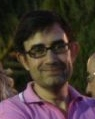
\includegraphics[width = 27
mm]{JJM.jpg},] \noindent\emph{JJ Merelo} es catedr\'{a}tico de Universidad
en el \'area de Arquitectura y Tecnolog\'{\i}a de Computadores, y
actualmente director de la Oficina de Software Libre de la UGR.
Mantiene un blog desde el a\~no 2002, y lo ha utilizado en clase desde
el a\~no 2004; tambi\'en wikis y, ultimamente, agregadores y otras
herramientas TIC. \'{U}ltimamente le ha dado por el \textsl{flipped
learning}, de lo que se informar\'{a} debidamente en esta columna.
\end{window}}}

\medskip

{\small{\begin{window}[0,r,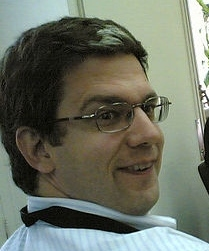
\includegraphics[width = 27 mm]{FTricas1.jpg},]
		\noindent  \emph{Fernando Tricas Garc\'{\i}a} es profesor
		titular de Lenguajes y Sistemas Inform\'aticos del Departamento
		de Inform\'atica e Ingenier\'{\i}a de Sistemas de la Universidad de
		Zaragoza.  Empez\'o a estudiar la blogosfera casi cuando a\'un no
		exist\'{\i}a (all\'a por el a\~no 2002) y a tratar de integrarla en los
		cursos y tareas docentes un poco despu\'es.  Ha impartido
		numerosas charlas relacionadas con el tema de la Web 2.0.
		Es actualmente Director de su departamento.  
		\end{window}}}

 \noindent mente
 diversos: a esto ayuda el tama\~no (no es f\'acil, en cuanto el
 equipo crece, que todas las personas tengan relaciones de amistad);
 esto tambi\'en refleja lo que seguramente nos suceder\'a
 posteriormente en el trabajo, donde no siempre podremos estar en el
 equipo con las personas m\'as afines.  Y puede ayudar al estudiantado
 a descubrir que hay gente interesante fuera de su c\'{\i}rculo.
 Tambi\'en conviene incidir en los procesos formales: por ejemplo, con
 reuniones internas del equipo (?`habr\'a actas?  ?`alg\'un otro
 mecanismo de seguimiento de los acuerdos adoptados?)  y con la
 persona responsable de la asignatura (preguntas relevantes sobre el
 proyecto, su organizaci\'on, ayudar a marcar hitos o actuar como
 ``cliente'', por ejemplo).  Otra pregunta puede hacerse relacionada con
 el momento.  Naturalmente, nadie nace ense\~nado: en muchas
 universidades se vienen utilizando asignaturas de proyectos para que
 los estudiantes tengan una aproximaci\'on informal (y conducida por
 la necesidad) antes de proporcionarles las herramientas necesarias
 (que vendr\'an en asignaturas posteriores).  Tal vez ser\'{\i}a
 posible intentar incluir este tipo de actividades en etapas m\'as
 tempranas o m\'as adelante, como refuerzo de aspectos ya aprendidos.
 En cuanto a qu\'e asignaturas coordinar es dif\'{\i}cil dar un
 consejo gen\'erico: a lo mejor podemos empezar con unas pocas (dos, o
 tres asignaturas que proponen un proyecto com\'un) y ver si se puede
 crecer (con la ventaja de que, seguramente, no supone un cambio del
 plan de estudios y su correspondiente proceso de verificaci\'on);
 pero tambi\'en se puede apostar por asignaturas dedicadas
 exclusivamente a esta tarea, que pueden enfocarse en materias
 concretas o ser mucho m\'as transversales.  En resumen, ser\'{\i}a
 conveniente que los profesores tuvieran, al menos conocimiento de
 estas metodolog\'{\i}as de desarrollo y trataran de que el alumno los
 aprendiera en entornos simulados, pero tan cercanos como sea posible
 a la realidad.

\bigskip

\noindent\emph{Todas las columnas de la serie Docencia 2.0
pueden descargarse en formato LaTeX desde
{\small\url{https://github.com/ReVision-Docencia-20/Columnas}}}

\noindent\rule{90mm}{1pt}

{\small \noindent
\includegraphics[height = 4ex]{CC.jpg} 2015 JJ. Merelo, F. Tricas. Este art\'{\i}culo es de acceso libre distribuido bajo los t\'erminos
de la Licencia Creative Commons de Atribuci\'on, que permite copiar,
distribuir y comunicar p\'ublicamente la obra en cualquier medio, s\'olido
o electr\'onico, siempre que se acrediten a los autores y fuentes
originales}


% \begin{thebibliography}{9}
% 	\bibitem{WA} John Paczkowski: \emph{WhatsApp: Bigger Than Twitter}.
% {\small\url{http://allthingsd.com/20130416/whatsapp-bigger-than-twitter/}},
% consultado en abril de 2013.}
% 
% \bibitem{Micr} Europa Press: Microsoft confirma la
% desaparici�n de Messenger y su integraci�n en Skype.
% {\small\texttt{http://www.europapress.es/portaltic/social 
% media/noticia-microsoft-confirma-desapari
% cion-messenger-integracion-skype-20121106
% 194539.html}},
% consultado en abril de 2013.
% 
% \bibitem{MT} Juan J. Merelo, F. Tricas:  \emph{Los medios y los memes.} En La
% Comunicaci�n Digital, editado por Germ�n Llorca Abad, Mar Iglesias
% Garc�a, �lvar Peris Blanes.  Tirant lo Blanc.  Valencia, Espa�a.
% pp.~219 -- 226.  2012.
% 
% \end{thebibliography}
\end{multicols}
\end{document}
	








\end{multicols}
\end{document}
�
